\chapter{Creating Robotic Arm}

\section{OpenSCAD}
OpenSCAD is an open source sriped based CAD program with which we decided to create our model of the robotic arm.\\
The softwar looks like this:\\
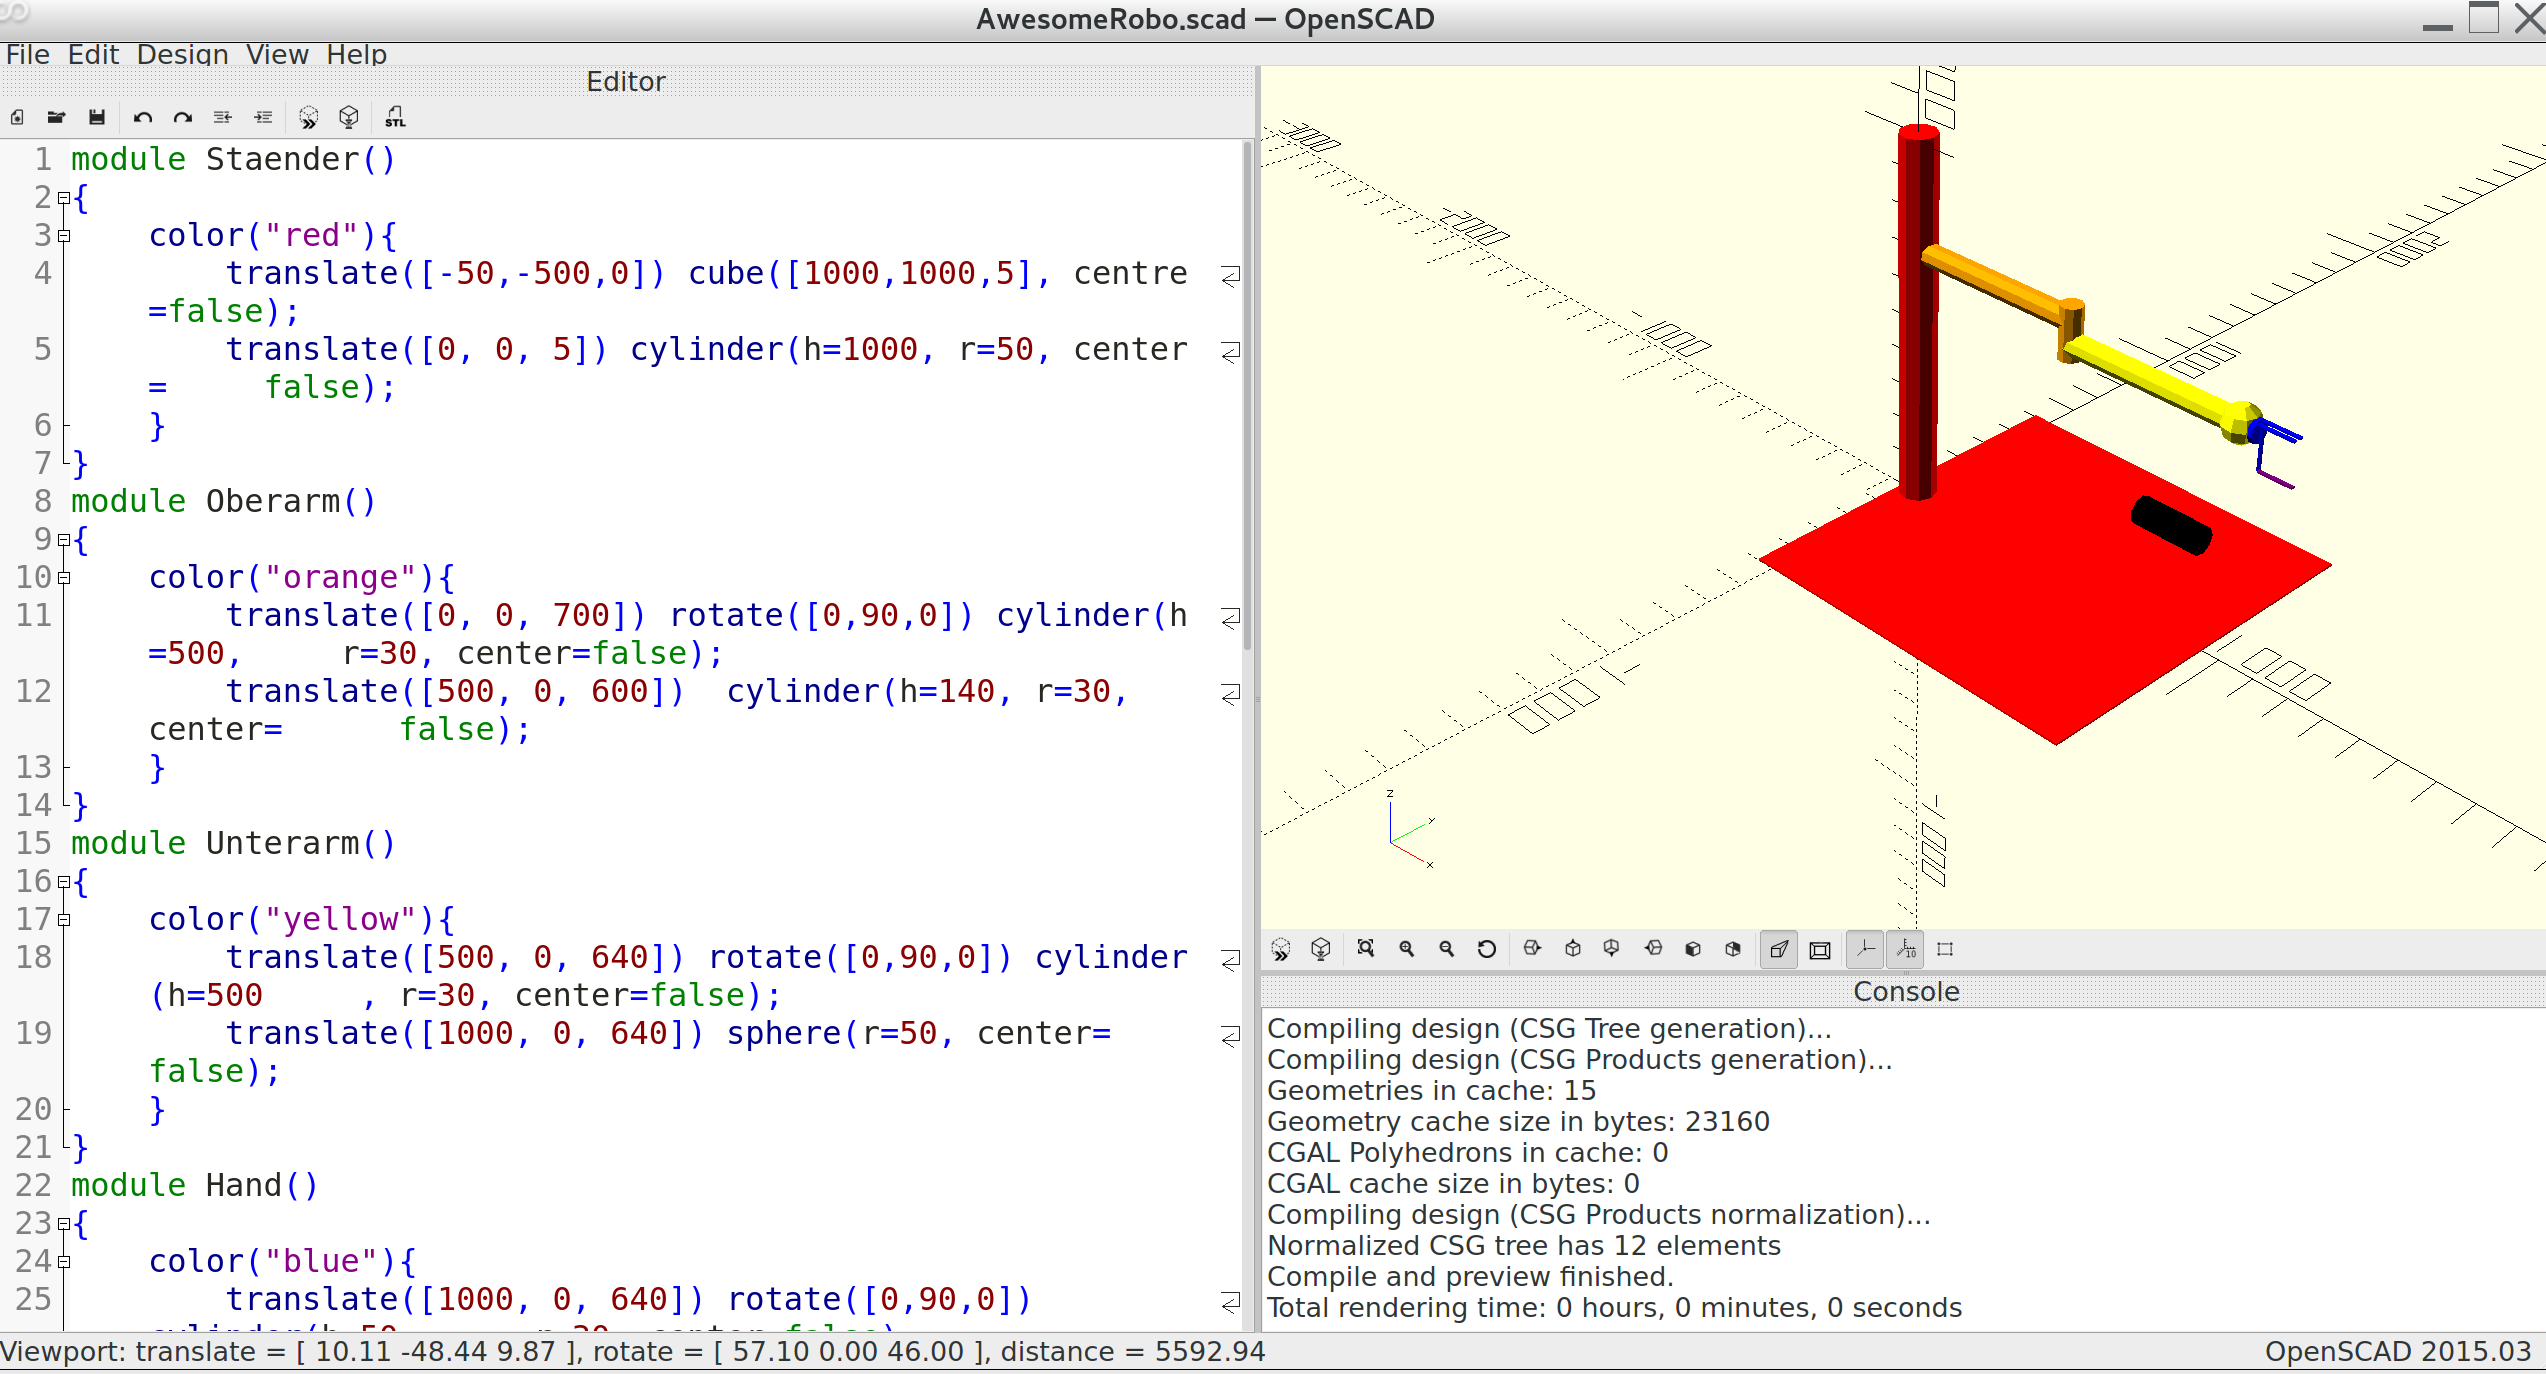
\includegraphics[width=\textwidth]{imgs/OpenSCAD/SoftwareWindow.png}
We collored all the different parts of the robotic arm in different collors for a better overview. All this parts are discribed in the following chapters.\\
As can be seen in the picture with OpenSCAD you can create modules seperately and place them where you want them. So you can add additional modules easily.

\section{Description of the Robotic Arm}
Our robotic arm is built up of 5 pieces. The pillar, the upper arm, the forearm, an hand with two fingers and a separate finger to squeeze.
Each of this part has their own movement possibilities:\\
- pillar:		no movement\\
- upper arm:	just z movement\\
- forearm:		just rotate around z-achsis\\
- hand:			rotate around all three achsises\\
- finger:		just z movement (but it depends on the posision of the hand)
\section{Exporting .stl-files}
Creating an .stl-file is a very easy task with the OpenSCAD software and the way we built our robotic arm. Just draw and render the modules separately. Then click File->Export->Export STL... Give it a name and click Save and that's it.
\pagebreak